\section{Results and discussion}

\begin{comment}
This section should include your main findings, properly presented with the aid of professional graphical devices (figures, graphs, tables, …). Results must be interpreted to ease the reader’s understanding of their significance and the findings should be linked to the research gaps and objectives identified in the first part of this document.

This section should be about \textbf{15-20 pages} long.
\end{comment}

\subsection{Impact of Thermal Camera/ Tripod Positioning on Vortex Generator Results}
As detailed in Section 3.3.1, this thesis involved the measurement of photovoltaic module temperature change for the following case: 15 mm cylindrical vortex generators placed on the underside of the photovoltaic module with a span-wise spacing of 51 mm and a stream-wise spacing of 79 mm. The cylindrical vortex generator was observed to be the most promising shape for optimal cooling performance according to a study by I.R. Chaudhury titled \textit{The cooling effects of vortex generators to increase efficiency on photovoltaic modules under forced convection} \cite{Chaudhury2024}. Furthermore, the 51 mm by 79 mm spacing configuration was also observed to be the most effective at cooling photovoltaic modules in a study by Z. Zhou titled \textit{Spacing Effect of Vortex Generator Array on PV Module Cooling in Forced Convection} \cite{Zhou2024}. Their findings are summarised in Table \ref{tab:past_experimental_findings}, with full details in Appendix~D.\par

\renewcommand{\arraystretch}{0.9}
\begin{table}[H]
    \centering
    \caption{Zhou et al. and Chaudhury et al.'s results for the following test case: 15 mm cylindrical vortex generators placed on the underside of the photovoltaic module with a span-wise spacing of 51 mm and a stream-wise spacing of 79 mm. Note: A positive value in the \textit{PV Module Temperature Change} column indicates cooling \cite{Chaudhury2024, Zhou2024}.}
    \resizebox{\textwidth}{!}{%
    \begin{tabular}{lcc}
        \toprule
        \textbf{Experimental Result Lead} & \textbf{Wind Speed (m/s)} & \textbf{PV Module Temperature Change ($^\circ$C)} \\
        \midrule
        \multirow{3}{*}{Z. Zhou} & 1 & 1.31 \\
                                & 2 & 2.15 \\
                                & 3 & 2.51 \\
        \midrule
        \multirow{3}{*}{I.R. Chaudhury} & 1 & 1.17 \\
                                & 2 & 2.10 \\
                                & 3 & 2.68 \\
        \bottomrule
    \end{tabular}%
    }
    \label{tab:past_experimental_findings}
    \vspace{-1em}
\end{table}
\renewcommand{\arraystretch}{1}

\begin{wrapfigure}{r}{0.5\linewidth}  % 'l' for left, adjust width as needed
    \vspace{-1em}
    \centering
    \includegraphics[width=\linewidth]{Figures/previous_results_vs_current_results.pdf}
    \vspace{-2.25em}
    \caption{Comparison of past photovoltaic module temperature change ($\Delta T$) and current with the results from this thesis, where the thermal camera was positioned to the side of the module.}
    \label{fig:previous_results_vs_current_results}
    \vspace{-2em}
\end{wrapfigure}

In addition to the performance-based justification for the selected vortex generator shape and spacing configuration, this experimental setup replicates that of Zhou et al. and Chaudhury et al., allowing for result confirmation. Thus, the first aim of this thesis was to confirm previous results surrounding the ability of cylindrical vortex generators to reduce the temperature of photovoltaic modules. However, during this thesis' experimental testing campaign, the previous results recorded by Zhou et al. and Chaudhury et al. could not be replicated when the thermal camera was positioned to the side of the photovoltaic module (Figure \ref{fig:side_tripod}). As shown in Figure \ref{fig:previous_results_vs_current_results}, while Chaudhury et al. and Zhou et al. observed the photovoltaic module to cool at a quasi-linear rate with increasing wind speed under the influence of 15 mm cylindrical vortex generators, the results from this thesis, when the thermal camera was positioned to the side, indicate that the module cooled at a rate that appears inversely proportional to wind speed. The results reported by Zhou et al. and Chaudhury et al. could only be closely replicated when the thermal camera was positioned directly in front of the photovoltaic module (Figure \ref{fig:centred_tripod}), also shown in Figure \ref{fig:previous_results_vs_current_results}.\par

\begin{figure}[H]
    \centering
    \begin{minipage}[b]{0.48\linewidth}
        \centering
        \includegraphics[height=8cm, width=\linewidth]{Figures/replace_side_tripod.jpg}
        \caption{Image of the thermal camera positioned to the side of the photovoltaic module.}
        \label{fig:side_tripod}
    \end{minipage}
    \hfill
    \begin{minipage}[b]{0.48\linewidth}
        \centering
        \includegraphics[height=8cm, width=\linewidth]{Figures/replace_centred_tripod.jpg}
        \caption{Image of the thermal camera and tripod positioned directly in front of the photovoltaic module.}
        \label{fig:centred_tripod}
    \end{minipage}
    \vspace{-1em}
\end{figure}
Therefore, it is believed that positioning the thermal camera directly in front of the photovoltaic module interferes with the approaching airflow, as the cylindrical tripod supporting the camera acts as a vortex generator. As shown in Figure \ref{fig:vortex_generator} of Section 2.4, positioning the tripod within the wind tunnel results in the formation of a forward stagnation point, boundary layer, and separation point along its surface, leading to the generation of Kármán vortices that induce turbulence and enhance mixing.

\begin{figure}[ht]
    \centering
    \begin{minipage}[t]{0.48\textwidth}
        \centering
        \includegraphics[width=\linewidth, height=3.4cm, trim=0 30 0 20, clip]{Figures/karman_vortex_street.png}
        \caption{A Kármán vortex street behind a cylinder at Re = 140. \cite{taneda_karman_1988}.}
        \label{fig:karman_vortex_street}
    \end{minipage}
    \hfill
    \begin{minipage}[t]{0.48\textwidth}
        \centering
        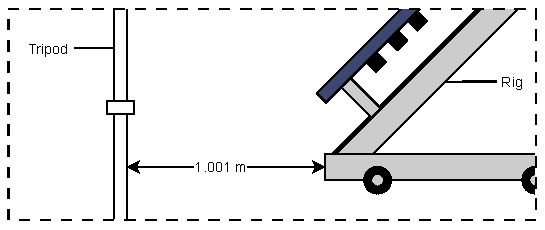
\includegraphics[width=\linewidth, trim=3 4 3 4, clip]{Figures/tripod_rig_distance.pdf}
        \caption{Perpendicular distance between the tripod and the experimental rig.}
        \label{fig:tripod_rig_distance}
    \end{minipage}
\end{figure}

Provided the Kármán vortex street (Figure \ref{fig:karman_vortex_street}) is sufficiently strong, the resulting turbulence would propagate across the 1.001 m perpendicular distance from the tripod’s position to the photovoltaic module (Figure \ref{fig:tripod_rig_distance}), thereby enhancing heat transfer primarily from the top surface of the module to the surrounding environment.

\subsubsection{Tripod Position Effect on Photovoltaic Module Temperature: A Theoretical Confirmation}
As shown in Equation 14, the Reynolds number for different wind speeds can be calculated using the wind speed, the tripod diameter, and the fluid's kinematic viscosity.
\begin{equation*}
\begin{tabular*}{\textwidth}{@{\extracolsep{\fill}} c c c @{}}
$\mathrm{Re_{D, 1\,m/s}} = \dfrac{1\,\mathrm{m/s} \times 0.032\,\mathrm{m}}{1.5 \times 10^{-5}\,\mathrm{m^2/s}} \approx 2133$ &
$\mathrm{Re_{D, 2\,m/s}} = \dfrac{2\,\mathrm{m/s} \times 0.032\,\mathrm{m}}{1.5 \times 10^{-5}\,\mathrm{m^2/s}} \approx 4267$ &
$\mathrm{Re_{D, 3\,m/s}} = \dfrac{3\,\mathrm{m/s} \times 0.032\,\mathrm{m}}{1.5 \times 10^{-5}\,\mathrm{m^2/s}} \approx 6400$
\end{tabular*}
\end{equation*}
All tested wind speeds produce subcritical Reynolds numbers, leading to Kármán vortex shedding in the wake. Based on empirical correlations, the laminar wake length behind a circular cylinder is approximately 5–10 times the cylinder diameter \cite{white1999fluid}. Consequently, the turbulent wake is expected to extend between 0.16 m and 0.32 m.
\begin{equation*}
    L_\mathrm{wake, laminar} \approx (5\ \mathrm{to}\ 10)\times D = (0.16\ \mathrm{to}\ 0.32)\ \mathrm{m}
\end{equation*}
Once the vortices are established, the turbulent wake can extend 10 to 50 times the diameter of the cylinder \cite{white1999fluid}.
\begin{equation*}
    L_\mathrm{wake, turbulent} \approx (10\ \mathrm{to}\ 50)\times D = (0.32\ \mathrm{to}\ 1.6)\ \mathrm{m}
\end{equation*}
Therefore, at a distance of 1.001 m from the tripod, the photovoltaic module resides within the cylinder’s wake, where it is expected to undergo increased mixing and convective cooling.

\subsubsection{Tripod Position Effect on Photovoltaic Module Temperature: An Experimental Confirmation}
To experimentally determine whether the tripod’s position affects module temperature, infrared images were examined with the tripod placed directly in front of the module and to its side.
\begin{figure}[H]
    \centering
    \begin{minipage}[b]{0.48\linewidth}
        \centering
        \includegraphics[height=9.7cm, width=\linewidth]{Figures/IR_image_side_tripod.jpg}
        \caption{Infrared image of the photovoltaic module taken to the side of the module.}
        \label{fig:IR_image_side_tripod}
    \end{minipage}
    \hfill
    \begin{minipage}[b]{0.48\linewidth}
        \centering
        \includegraphics[height=9.7cm, width=\linewidth]{Figures/IR_image_centred_tripod.jpg}
        \caption{Infrared image of the photovoltaic module taken directly in front of the module.}
        \label{fig:IR_image_centred_tripod}
    \end{minipage}
\end{figure}

The infrared image captured from the front-facing position (Figure \ref{fig:IR_image_centred_tripod}) displays a distinct yellow streak through the centre of the module, which is absent in the infrared image taken when the camera was positioned to the side of the module (Figure \ref{fig:IR_image_side_tripod}). Through an observation of the temperature gradient tool positioned to the right of the photovoltaic module in Figure \ref{fig:IR_image_side_tripod} and Figure \ref{fig:IR_image_centred_tripod}, it is evident that the yellow streak indicates localised cooling across the centre of the photovoltaic module. Furthermore, the position of this localised cooling aligns with the location of the thermal camera during testing, and is not present in the infrared image taken when the tripod and thermal camera were positioned to the side of the module. Thus, this observation indicates that the tripod disrupted airflow, creating turbulence and enhancing cooling of the module surface.

As a result of this analysis, the infrared camera and tripod were moved to the side of the photovoltaic module for all tests, preventing tripod-generated vortices from affecting the module temperature. Furthermore, the temperature measurements reported by Zhou et al. and Chaudhury et al. might need to be revised, as their experiments did not take into account the cooling effects caused by the centrally positioned tripod and thermal camera. However, since this setup was the same in all their trials, the optimal spacing and vortex-generator shape they identified are likely still valid and unaffected by this oversight.

\subsection{Impact of Ambient Temperature on Vortex Generator Results}
The main aim of this thesis was to determine the vortex generator height that maximises the reduction in photovoltaic module temperature and, consequently, the increase in its electrical efficiency. Unexpectedly, the 15 mm vortex generator array yielded inconsistent outcomes during the testing campaign, with certain cases exhibiting slight heating relative to the baseline and others exhibiting slight cooling under identical wind speed conditions.

\begin{wrapfigure}{r}{0.65\linewidth} % 'r' = right, '0.6\linewidth' = figure width
    \vspace{-1.25em}
    \centering
    \includegraphics[width=\linewidth, trim=0 0 0 0, clip]{Figures/h15_vs_baseline.pdf}
    \vspace{-1.95em}
    \caption{Photovoltaic module temperature as a function of ambient temperature at wind speeds of 1 m/s, 2 m/s, and 3 m/s, showing the effect of a 15 mm vortex generator array.}
    \label{fig:h15_vs_baseline}
    \vspace{-2em}
\end{wrapfigure}

To examine these variations in photovoltaic module temperature under identical wind speeds, the module temperature was plotted against ambient temperature on the baseline trend graph, as shown in Figure \ref{fig:h15_vs_baseline}. Figure \ref{fig:h15_vs_baseline} reveals a linear relationship between ambient temperature and the photovoltaic module temperature when subjected to the 15 mm vortex generator array. However, this linear relationship demonstrated a reduced gradient of approximately 0.9, compared to the baseline gradient values, which ranged from 1.2 to 1.3. This difference led to the vortex generator line of best fit intersecting the baseline line of best fit across all three wind speeds, resolving the initial confusion over the seemingly inconsistent results. Trend-line equations are provided in Appendix D.

\subsubsection{The Impact of Vortex Generators on Photovoltaic Module Temperature Changes under Varying Ambient Temperature Conditions: An Explanation}
The observed relationship between vortex generators and photovoltaic module temperature reduction, influenced by ambient temperature, was crucial in explaining the variability seen during repeated experimental tests. However, it is also essential to understand why vortex generators caused the module to heat up at lower ambient temperatures while cooling it at higher ambient temperatures.

% Overview of the energy balance equations
% Justification for why this case was chosen for the energy balance equation
To investigate the influence of vortex generators on photovoltaic module temperature under different ambient conditions, energy balance equations were developed for the 15~mm vortex generator configuration and its corresponding baseline case at ambient temperatures of 19.9~$^\circ$C and 25.5~$^\circ$C, both subjected to a forced-convection velocity of 1~m/s. These temperatures were selected because the vortex generators were observed to increase module temperature at 19.9~$^\circ$C but reduce it at 25.5~$^\circ$C. Furthermore, the 15~mm case was chosen over the 75~mm configuration due to the larger volume of experimental data available. Moreover, because the behaviour at 1~m/s closely matches that observed at 2~m/s and 3~m/s, the energy balance trends established for the 1~m/s condition are also applicable to the higher flow velocities.
\begin{table}[H]
    \centering
    \caption{Summary of the heat-loss components used in the energy-balance equations for the 15~mm vortex generator and baseline configurations at 19.9~$^\circ$C and 25.5~$^\circ$C. Full derivations are provided in Appendix~D.}
    \resizebox{\textwidth}{!}{%
    \begin{tabular}{ccccccc}\toprule
         \textbf{Case} &  $\dot{Q}_\mathrm{conv,top}\ (\mathrm{W})$ &  $\dot{Q}_\mathrm{conv,bottom}\ (\mathrm{W})$ &  $\dot{Q}_\mathrm{rad,top}\ (\mathrm{W})$ &  $\dot{Q}_\mathrm{rad,bottom}\ (\mathrm{W})$ &$\dot{Q}_\mathrm{cond,array}\ (\mathrm{W})$ &$\dot{Q}_\mathrm{loss}\ (\mathrm{W})$ \\\midrule
         Baseline (19.9 $^\circ$C) & 185.31& 185.31& 250.90&   242.35&-&863.86\\ 
         15 mm VG (19.9 $^\circ$C) & 194.45& 127.36& 262.53&  246.11&33.42&863.86\\
 Baseline (25.5 $^\circ$C) & 196.26& 196.26& 280.61& 271.04& -&944.16\\
         15 mm VG (25.5 $^\circ$C) & 193.35& 173.50& 276.69&  267.26&33.37&944.16\\ \bottomrule
    \end{tabular}
    }
    \label{tab:energy_balance_summary_table}
\end{table}
% Energy Balance Equation is in Agreement with Experimental Measurements (Lower Ambient Temperature)
As shown in Table~\ref{tab:energy_balance_summary_table}, at an ambient temperature of 19.9~$^\circ$C, all heat-transfer components are greater for the vortex generator case than for the baseline case, except for the convective heat transfer at the bottom surface of the photovoltaic module, $\dot{Q}_\mathrm{conv,bottom}$. Therefore, since the vortex generator array increases the photovoltaic module temperature at lower ambient temperatures, as shown in Figure~\ref{fig:h15_vs_baseline}, this rise in module temperature can be attributed to the substantial reduction in convective heat transfer at the bottom surface of the module, which decreases from 185.31~W for the baseline case to 127.36~W for the 15~mm vortex generator case. The convective heat transfer from the bottom surface of the photovoltaic module depends on the bottom-surface area, $A_\mathrm{s}$, the module and ambient temperatures, ($T_\mathrm{mod}$$-$ $T_\mathrm{amb}$), and the convective heat-transfer coefficient, $h_\mathrm{conv,bottom}$, as shown in Equation~9 \cite{engel2014IntroductionAndBasicConcepts}. The temperature difference, ($T_\mathrm{mod} - T_\mathrm{amb}$), was nearly identical for both the baseline and vortex-generator cases, and the bottom-surface area was the same for both configurations. Consequently, the reduction in convective heat transfer arises from a lower bottom-surface convective heat transfer coefficient, $h_\mathrm{conv,bottom}$. Appendix~D shows that the 15~mm array yields a coefficient of 2.23~$\mathrm{W\,m^{-2}\,K^{-1}}$, compared with 4.24~$\mathrm{W\,m^{-2}\,K^{-1}}$ for the baseline case.

As the ambient temperature increases from 19.9~$^\circ$C to 25.5~$^\circ$C, Figure~\ref{fig:h15_vs_baseline} shows a transition in which the 15~mm vortex generator array shifts from heating the module to cooling it. The energy-balance calculations for the 15~mm vortex generator and corresponding baseline cases at 25.5~$^\circ$C indicate that this cooling effect is driven primarily by an increase in convective heat-transfer from the bottom surface of the module. The conductive heat transferred from the module to the vortex generators changes only marginally with ambient temperature and therefore does not meaningfully contribute to the observed transition. Thus, the dominant factor is the increase in the bottom-surface convective heat transfer coefficient with rising ambient temperature, with $h_\mathrm{conv,bottom}$ increasing from 2.23~$\mathrm{W\,m^{-2}\,K^{-1}}$ at 19.9~$^\circ$C to 3.81~$\mathrm{W\,m^{-2}\,K^{-1}}$ at 25.5~$^\circ$C for the 15~mm array.

Therefore, to explain why the vortex generators increase photovoltaic module temperature at low ambient temperatures but reduce module temperature at higher ambient temperatures, it is necessary to identify why rising ambient temperature causes an increase in the bottom-surface convective heat transfer coefficient, $h_\mathrm{conv,bottom}$.
\begin{figure}[H]
    \centering
    \includegraphics[width=\linewidth, trim=0 200 0 0, clip]{Figures/cfd_h15_222.png}
    \caption{CFD analysis of the experimental rig for the 15~mm vortex-generator array under 1~m/s airflow at an ambient temperature of 22.2~$^\circ$C.}
    \label{fig:cfd_h15_222}
\end{figure}
\begin{figure}[H]
    \centering
    \includegraphics[width=\linewidth]{Figures/cfd_h15_261.png}
    \caption{CFD analysis of the experimental rig for the 15~mm vortex-generator array under 1~m/s airflow at an ambient temperature of 26.1~$^\circ$C.}
    \label{fig:cfd_h15_261}
    \vspace{-1em}
\end{figure}
As a means of validating the experimental results presented in Figure~\ref{fig:h15_vs_baseline}, CFD analyses of the experimental rig operating under 1~m/s airflow were performed for the 15~mm vortex-generator case at ambient temperatures of 22.2~$^\circ$C (Figure~\ref{fig:cfd_h15_222}) and 26.1~$^\circ$C (Figure~\ref{fig:cfd_h15_261}) by PhD candidate Matthew Deng. The simulations showed that the vortex generators installed on the underside of the panel produced recirculation wakes, which are zones of reversed or disturbed flow that form immediately downstream of each generator due to flow separation \cite{Taylor2011Recirculation}. As illustrated in Figure~\ref{fig:cfd_h15_222}, the wakes confine warmer air near the photovoltaic module, whereas the wakes in Figure~\ref{fig:cfd_h15_261} appear slightly weaker, suggesting marginally reduced heat retention at the higher ambient temperature. While this behaviour aligns with the observed increase in bottom-surface convection at higher ambient temperatures, the magnitude of the difference is small and the CFD results therefore serve as qualitative rather than definitive support for the experimental trends.

Recent baseline tests conducted at higher ambient temperatures produced photovoltaic module temperatures that were approximately 1.4~$^\circ$C lower than the expected baseline results across all wind speeds, as shown in Figure~\ref{fig:h15_vs_baseline_vs_new_data}.
\begin{wrapfigure}{r}{0.65\linewidth}
    \vspace{-0.5em}
    \centering
    \includegraphics[width=1\linewidth]{Figures/h15_vs_baseline_vs_new_data.pdf}
    \vspace{-2em}
    \caption{Comparison of original baseline trends, new baseline data, and 15~mm vortex-generator results across all wind speeds.}
    \label{fig:h15_vs_baseline_vs_new_data}
    \vspace{-2em}
\end{wrapfigure}
% the baseline is lower / what to do next
This difference may be attributed to variations in equipment positioning, as the earlier baseline tests were conducted before the influence of the thermal camera and tripod on the measured module temperature was understood. The relevance of this observation to the influence of ambient temperature on the vortex-generator results arises from the fact that the baseline cases were originally confirmed only at lower ambient temperatures due to environmental constraints. If the recently observed reduction in baseline photovoltaic module temperature at higher ambient temperatures (Figure~\ref{fig:h15_vs_baseline_vs_new_data}) is consistently reproduced, the gradients of the baseline trends at all wind speeds would decrease. This would shift the baseline trend lines toward being parallel with the vortex-generator trends and clarify the influence of ambient temperature on result interpretation, potentially removing the apparent transition from module heating to cooling.

The discovery of ambient temperature’s influence on photovoltaic module temperature changes led to a refinement in determining the optimal vortex generator height. Rather than simply comparing the temperature change, $\Delta T$, across different vortex generator heights, it became necessary to ensure consistent ambient temperatures to draw valid conclusions about which height most effectively reduces module temperature. As a result, experimental tests at varying ambient temperatures were conducted for all vortex generator heights to generate reliable trend lines.

\subsection{Experimental Vortex Generator Height Results}
Applying the refined method for determining the optimal vortex generator height, the 75~mm array was evaluated against the 15~mm array, as shown in Figure~\ref{fig:h15_vs_h75_vs_baseline}. Although the 150~mm vortex generator array was tested experimentally during this thesis campaign, its results could not be replicated or validated due to experimental rig limitations and time constraints, as discussed in the outliers section below. Thus, Figure \ref{fig:h15_vs_h75_vs_baseline} reveals the 15~mm vortex generator array to be the most effective at reducing photovoltaic module temperature at elevated ambient temperatures across all wind speeds. Furthermore, at lower ambient temperatures, the 15~mm vortex generator array produces the smallest increase in module temperature when compared with the 75~mm array. The numerical values corresponding to Figure~\ref{fig:h15_vs_h75_vs_baseline} are consolidated in Table~\ref{tab:results_summary}, located in Appendix~D.

\begin{figure}[H]
    \centering
    \includegraphics[width=\linewidth]{Figures/h15_vs_h75_vs_baseline.pdf}
    \vspace{-2em}
    \caption{Photovoltaic module temperature versus ambient temperature at wind speeds of 1~m/s, 2~m/s, and 3~m/s, comparing the temperature reduction effects of 15~mm, 75~mm, and 150~mm vortex generator arrays.}
    \label{fig:h15_vs_h75_vs_baseline}
    \vspace{-1.5em}
\end{figure}

% 1 m/s
At a wind speed of 1 m/s, the 15 mm vortex generator array increased the temperature of the photovoltaic module by 1.12 $^\circ$C when the ambient temperature was 19.87 $^\circ$C. As the ambient temperature rises, the heating effect of the vortex generator diminishes linearly until the ambient temperature reaches 24.38 $^\circ$C. Beyond this point, the photovoltaic module begins to cool under the influence of the 15 mm vortex generator array. This cooling continues at a linear rate, reaching a reduction of 0.36 $^\circ$C at an ambient temperature of 25.50 $^\circ$C. Similarly, at a wind speed of 1 m/s, the 75 mm vortex generator array increases the photovoltaic module temperature by 1.41 $^\circ$C when the ambient temperature is 22.27 $^\circ$C, approximately 0.75 $^\circ$C more than the heating caused by the 15 mm vortex generator array at the same ambient temperature. The heating effect of the 75 mm vortex generator array also decreases linearly until the ambient temperature reaches 25.90 $^\circ$C. Beyond this point, as the ambient temperature continues to rise, the photovoltaic module begins to cool at a linear rate, with a cooling of 0.98 $^\circ$C observed at an ambient temperature of 28.13 $^\circ$C. Thus, at 1 m/s, the 15~mm array heats the module less at low ambient temperatures and cools it more effectively at higher temperatures.

% 2 m/s
At a 2 m/s wind speed, the 15 mm vortex generator array raised the photovoltaic module temperature by 1.08 $^\circ$C at an ambient temperature of 20.60 $^\circ$C. As the ambient temperature increases to 23.47 $^\circ$C, the heating effect on the photovoltaic module gradually decreases at a linear rate. Beyond 23.47 $^\circ$C, the module begins to cool at an increasing linear rate, reaching 0.79 $^\circ$C of cooling at an ambient temperature of 25.80 $^\circ$C. The 75 mm vortex generator array exhibits a similar relationship, increasing the photovoltaic module temperature by 1.43 $^\circ$C at an ambient temperature of 23.10 $^\circ$C, approximately 1.40 $^\circ$C more than the heating caused by the 15 mm vortex generator array at the same ambient temperature. As the ambient temperature increases, the magnitude of heating caused by the 75 mm vortex generator array decreases at a linear rate until the ambient temperature reaches 26.47 $^\circ$C. As the ambient temperature increases past this point, the module transitions into a clear linear cooling trend, reaching a 1.19 $^\circ$C reduction at 28.9 $^\circ$C. Hence, at 2~m/s, the 15~mm array outperforms the 75~mm array by causing less heating at low ambient temperatures and delivering greater cooling at higher temperatures.

% 3 m/s
At a wind speed of 3 m/s, the trend lines for both the 15 mm and 75 mm vortex generator arrays exhibit similar characteristics to those observed at 1 m/s and 2 m/s. The 15 mm vortex generator array raises the photovoltaic module temperature by 0.88 $^\circ$C at an ambient temperature of 21.57 $^\circ$C. As the ambient temperature increases to 24.21 $^\circ$C, the heating effect of the 15 mm vortex generator array diminishes linearly. Beyond 24.21 $^\circ$C, the photovoltaic module begins to cool at an increasing linear rate, reaching a cooling of 0.99 $^\circ$C at an ambient temperature of 26.70 $^\circ$C. The 75 mm vortex generator array increases the photovoltaic module temperature by 1.30 $^\circ$C at an ambient temperature of 24.13 $^\circ$C, approximately 1.30 $^\circ$C higher than the heating caused by the 15 mm vortex generator array at the same ambient temperature. As the ambient temperature rises, the heating effect of the 75 mm vortex generator array decreases at a linear rate until the ambient temperature reaches 27.80 $^\circ$C. Once the ambient temperature exceeds past this point, the module enters a linear cooling trend, reaching a 1.05 $^\circ$C reduction at 30 $^\circ$C. Thus, at 3 m/s, the 15 mm vortex generator array heats the module less than the 75 mm vortex generator array at lower ambient temperatures and provides more effective cooling as the temperature increases.

\subsubsection{Experimental Vortex Generator Height Result Outliers}
At a wind speed of 1~m/s, the 75~mm vortex generator array tested on 17~September~2025 reduced the photovoltaic module temperature by 2.28~$^\circ$C, which exceeded the cooling achieved by the 15~mm vortex generator array. This behaviour was not observed at wind speeds of 2~m/s or 3~m/s. It is important to note that the 1~m/s result originates from a single experimental run at a specific ambient condition, and thus requires cautious interpretation. Given the established trends at 2~m/s and 3~m/s, this anomaly warranted further investigation. Consequently, additional experimental tests were performed at higher ambient temperatures for the vortex generator array, which demonstrated cooling of approximately 1~$^\circ$C across all wind speeds. Given its anomalous and non-repeatable behaviour, the data point was excluded from the 1~m/s vortex generator trend line shown in Figure \ref{fig:h15_vs_h75_vs_baseline}. Further testing of the 75~mm array at higher ambient temperatures is recommended to better validate its thermal performance.

A single experimental test was conducted using the 150~mm vortex generators. As shown in Figure~\ref{fig:h15_vs_h75_vs_baseline}, the recorded data indicated cooling of 2.52~$^\circ$C at 1~m/s, 1.56~$^\circ$C at 2~m/s, and 1.15~$^\circ$C at 3~m/s. However, due to constraints of the experimental rig, the 150~mm vortex generators were attached to the acrylic roofing rather than to the underside of the photovoltaic module, as was done for the other vortex generator heights. The roofing exhibited noticeable sagging towards the centre of the photovoltaic module under its own weight, resulting in a non-negligible gap of approximately 10~mm between the module and the tips of the 150~mm vortex generators. Although the data from this test have been included in Figure~\ref{fig:h15_vs_h75_vs_baseline} for completeness, the measurements obtained under these conditions are considered unreliable given the compromised geometric configuration. To obtain valid 150~mm results, the acrylic roofing near the module centre must be reinforced to maintain a consistent 150~mm separation before further testing.

\subsubsection{Optimal Vortex Generator Height for Maximising Photovoltaic Module Temperature Reduction: An Explanation}
The identification of the 15 mm vortex generator as the optimal height for maximising photovoltaic module temperature reduction warrants an in-depth explanation, particularly given its seemingly contradictory stance to the findings presented in the literature review of this document.

\begin{table}[H]
    \centering
    \caption{Summary of heat-loss components in the energy-balance equations for the 15~mm and 75~mm vortex-generator cases at 19.9~$^\circ$C. Full derivations are provided in Appendix~D.}
    \resizebox{\textwidth}{!}{%
    \begin{tabular}{ccccccc}\toprule
         \textbf{Case} &  $\dot{Q}_\mathrm{conv,top}\ (\mathrm{W})$ &  $\dot{Q}_\mathrm{conv,bottom}\ (\mathrm{W})$ &  $\dot{Q}_\mathrm{rad,top}\ (\mathrm{W})$ &  $\dot{Q}_\mathrm{rad,bottom}\ (\mathrm{W})$ &$\dot{Q}_\mathrm{cond,array}\ (\mathrm{W})$ &$\dot{Q}_\mathrm{loss}\ (\mathrm{W})$ \\\midrule 
         15 mm VG Array& 194.45& 127.36& 262.53&  246.12&33.42&863.86\\
         75 mm VG Array& 200.92& 104.05& 270.75&  253.81&34.34&863.86\\ \bottomrule
    \end{tabular}
    }
    \label{tab:energy_balance_heights_summary_table}
    \vspace{-1em}
\end{table}
As shown in Table~\ref{tab:energy_balance_heights_summary_table}, the convective heat transfer from the top surface of the photovoltaic module, the radiative heat transfer from both the top and bottom surfaces, and the conductive heat transfer from the module to the vortex generator array are all greater for the 75~mm vortex generator case than for the 15~mm case. However, even with larger values for all other heat-transfer components, the 75~mm case still results in a higher module temperature. The derivations in Appendix~D indicate that this behaviour is driven by a markedly lower convective heat transfer from the bottom surface of the module for the 75~mm case, decreasing from 127.36~W for the 15~mm vortex generator array to 104.05~W for the 75~mm vortex generator array. The convective heat transfer from the bottom surface of the photovoltaic module can be expressed using Newton’s law of cooling, as shown in Equation~9~\cite{engel2014FundamentalsOfConvection}. The underside surface area of the module remained constant across all experimental cases, and the temperature difference between the module and the ambient air was nearly identical for both the 15~mm and 75~mm vortex generator configurations. Consequently, with all other variables known, the convective heat-transfer coefficients for both cases were determined, as presented in Appendix~D. These calculations show that the convective heat-transfer coefficient for the 75~mm array is lower, at 2.23~$\mathrm{W\,m^{-2}\,K^{-1}}$, compared with 2.80~$\mathrm{W\,m^{-2}\,K^{-1}}$ for the 15~mm array.
\begin{figure}[H]
    \centering
    \begin{minipage}[b]{0.48\linewidth}
        \centering
        \includegraphics[width=\linewidth, trim=20pt 15pt 25pt 10pt, clip]{Figures/mass_flow_rate_h15.pdf}
        \caption{Inlet geometry of the 15~mm vortex-generator rig. The inlet area was computed as $A = 0.999 \times 0.15 - 13 \times 0.015 \times 0.02 = 0.15\ \mathrm{m^2}$.}
        \label{fig:mass_flow_rate_h15}
    \end{minipage}
    \hfill
    \begin{minipage}[b]{0.48\linewidth}
        \centering
        \includegraphics[width=\linewidth, trim=20pt 15pt 25pt 10pt, clip]{Figures/mass_flow_rate_h75.pdf}
        \caption{Inlet geometry of the 75~mm vortex-generator rig. The inlet area was computed as $A = 0.999 \times 0.15 - 13 \times 0.075 \times 0.02 = 0.13\ \mathrm{m^2}$.}
        \label{fig:mass_flow_rate_h75}
    \end{minipage}
    \vspace{-1.5em}
\end{figure}
The reduced convective heat-transfer coefficient observed for the 75~mm case arises from the smaller cross-sectional flow area between the photovoltaic module and the acrylic roofing introduced by the increased vortex-generator height, as shown in Figure~\ref{fig:mass_flow_rate_h15} and Figure~\ref{fig:mass_flow_rate_h75}. This reduction in cross-sectional area, \(A\), lowers the mass flow rate of the incoming air, \(\dot{m}\), a behaviour consistent with confined-flow literature; Ekong~(2020) reported a clear decrease in the mass flow rate, \(\dot{m}\), with diminishing orifice diameter in controlled duct-flow experiments~\cite{Ekong2020Effect}. The relationship governing this dependence is expressed in Equation~19~\cite{engel2014IntroductionAndBasicConcepts}.
\begin{equation}
    \dot{m} = \rho A V
\end{equation}
The expression for the mass flow rate, $\dot{m}$, can be substituted into the Reynolds number definition (Equation~14), showing that the Reynolds number, $\mathrm{Re}$, is directly proportional to the mass flow rate, $\dot{m}$, as presented in Equation~20~\cite{engel2014ExternalForcedConvection}. Ekong reported a similar relationship, observing that the Reynolds number, $\mathrm{Re}$, increased proportionally with the mass flow rate, $\dot{m}$, such that a reduction in the mass flow rate, $\dot{m}$, led directly to a corresponding decrease in Reynolds number, $\mathrm{Re}$~\cite{Ekong2020Effect}.
\begin{equation}
    \mathrm{Re}=\frac{\dot{m}L_c}{A\mu}
\end{equation}
The proportional relationship between the Reynolds number, $\mathrm{Re}$, and the Nusselt number, $\mathrm{Nu}$, is well documented in existing literature~\cite{engel2014ExternalForcedConvection}. Accordingly, as shown in the generalised Nusselt number expression in Equation~21, a reduction in the Reynolds number, $\mathrm{Re}$, leads to a corresponding decrease in the Nusselt number, $\mathrm{Nu}$.
\begin{equation}
    \mathrm{Nu}=\mathrm{Re^m}\mathrm{Pr^n}
\end{equation}
Finally, the proportional relationship between the Nusselt number and the convective heat transfer coefficient, shown in Equation~13, indicates that increasing the vortex generator height reduces the convective heat transfer coefficient and, consequently, the convective heat transfer. Therefore, the conclusion that the reduced bottom surface convective heat transfer in the 75~mm case arises from the smaller cross-sectional flow area between the photovoltaic module and the acrylic roofing is both mathematically consistent and supported by existing experimental studies.
